\chapter{Автономный генератор}
\label{ch:chap3}
\section{Постановка задачи}
В этом задании нам нужно добиться желаемого выхода, в случае второго варианта он будет таковым:
$$
g_{wanted}(t) = g_w(t) = cos(-2t) + e^{6t}sin(5t)
$$
А получить желаемый сигнал нам нужно посредством подбора параметров $A, C, x(0)$ для системы вида:
$$
\begin{cases}
    \dot{x} = Ax, \\
    g = Cx;
\end{cases}
$$
Выход системы мы рассматриваем при свободном движении, и он должен будет совпасть с $g_w(t)$.

Проверку наших матриц с желаемым сигналом мы будем осуществлять с помощью следующей структурной схемы:
\begin{figure}[ht]
    \centering
    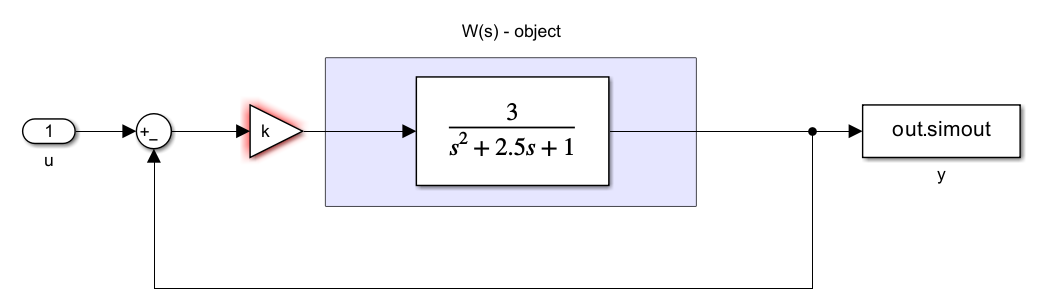
\includegraphics[width=1\textwidth]{scheme_system3.png}
	\caption{Структурная схема - проверка}
\end{figure}


\newpage
\section{Восстановление матриц}
Свободному движению систему соответствует следующая система:
$$
\begin{cases}
    x_{free}(t) = e^{At}x(0), \\
    y_{free}(t) = Ce^{At}x(0);
\end{cases}
$$, где матрицы $C,x(0)$ - параметры системы:
$$
    C = \feqvector[&]{c_1, c_2, c_3, c_4}, \tab x(0) = \feqvector{a_1, a_2, a_3, a_4}
$$
Пойдём методом "Жордана", для этого посмотрим какие характерестические корни соответствуют решению $g_w(t)$:
$$
\lambda_{1,2} = \pm2i, \tab \lambda_{3,4}=6\pm5i
$$, где первая пара корней соответствует косинусу, а вторая - экспонента с синусом. Тогда составим следующую Жорданову матрицу по корням:
$$
A = \begin{bmatrix}
      0 & +2 & 0 & 0  \\
      -2 & 0 & 0 & 0 \\
      0 & 0 & 6 & 5 \\
      0 & 0 & -5 & 6
    \end{bmatrix}
$$
Тогда возьмём матричную экспоненту, а после домножим на начальные условия:
$$
e^{At}x(0) = exp\bigg(\begin{bmatrix}
    0 & +2 & 0 & 0  \\
    -2 & 0 & 0 & 0 \\
    0 & 0 & 6 & 5 \\
    0 & 0 & -5 & 6
  \end{bmatrix}t\bigg) \feqvector{a_1,a_2,a_3,a_4}
$$
Упростим выражение:
$$
\begin{aligned}
    e^{At}x(0) = \begin{bmatrix}
        cos(-2t) & sin(-2t) & 0 & 0  \\
        -sin(-2t) & cos(-2t) & 0 & 0 \\
        0 & 0 & e^{6t}cos(5t) & e^{6t}sin(5t) \\
        0 & 0 & -e^{6t}sin(5t) & e^{6t}cos(5t)
      \end{bmatrix}\feqvector{a_1,a_2,a_3,a_4} = \dots \\  
      e^{At}x(0) = \feqvector{a_1cos(2t)-a_2sin(2t), a_1sin(2t) + a_2cos(2t), e^{6t}(a_3cos(5t)+a_4sin(5t)), e^{6t}(-a_3sin(5t)+a_4cos(5t))}
\end{aligned}
$$
Найдём выход системы:
$$
y_{free}(t) = Ce^{At}x(0) = \feqvector[&]{c_1, c_2, c_3, c_4}\feqvector{a_1cos(2t)-a_2sin(2t), a_1sin(2t) + a_2cos(2t), e^{6t}(a_3cos(5t)+a_4sin(5t)), e^{6t}(-a_3sin(5t)+a_4cos(5t))}
$$
$$
    \begin{aligned}
        y_{free}(t) = a_1c_1cos(2t) - c_1a_2sin(2t) + a_1c_2sin(2t) + c_2a_2cos(2t) + \\
        e^{6t}c_3(a_3cos(5t) + a_4sin(5t)) +e^{6t}c_4(a_4cos(5t) - a_3sin(5t))
    \end{aligned}
$$
Сгруппируем слагаемые несколько иным образом:
$$
    \begin{aligned}
        y_{free}(t) =  (a_1c_2 - c_1a_2)sin(2t) ( a_1c_1 + c_2a_2)cos(2t) + \\
        e^{6t}cos(5t)(c_3a_3 + c_4a_4) + e^{6t}sin(5t)(c_3a_4 - a_3c_4)
    \end{aligned}
$$
Посмотрим на желаемый выходной сигнал, и тогда предъявим следующие требования к коэффициентам:
$$
\begin{cases}
    a_1c_2 = a_2c_1 \\
    a_2c_2 + a_1c_1 = 1 \\
    a_3c_3 + a_4c_4 = 1 \\
    a_4c_3 = a_3c_4 
\end{cases}
$$
Как можно заметить, мы не сможем найти эти восемь коэффициентов единственным образом, здесь существуте бесконечное множество их комбинаций, поэтому просто выберем удобную:
$$
    C = \feqvector[&]{\frac{1}{5}, \frac{2}{5}, \frac{3}{25}, \frac{4}{25}}, \tab x(0) = \feqvector{1, 2, 3, 4}
$$
Мы смогли получить параметры $A, C, x(0)$, теперь подставим их в блок $State-Space$ симулинка, а после сравним с заданием $g_w(t)$ через матлабовскую функцию:
\begin{figure}[ht]
    \centering
    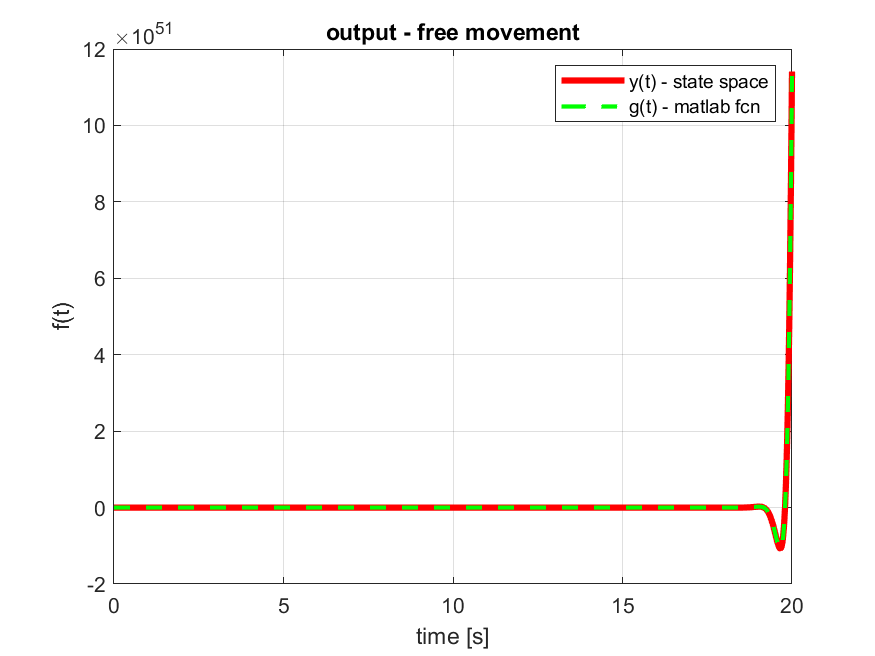
\includegraphics[width=1\textwidth]{output_task3.png}
	\caption{Симумляция - сравнение нашего сигнала с желаемым}
\end{figure}
Они совпали, это прекрасно!

\endinput